\documentclass{article}
\usepackage[utf8]{inputenc}
\usepackage{amsmath}
\usepackage{amssymb}
%\usepackage{pythontex}
\usepackage{minted}
\usepackage{xcolor} % to access the named colour LightGray
\usepackage{geometry} %to set page size
\usepackage{graphicx}
\usepackage{tcolorbox}


\title{Python Lab Notebook}
\author{Soumya Majhi}
\date{Sem-4 2022}

\geometry{a4paper,
 %total={170mm,257mm},
 left=30mm,
 right=20mm,
 top=30mm,
 bottom=30mm
 }


\begin{document}

\maketitle
\thispagestyle{empty}
% \begin{table}[H]
%     \begin{center}
%         \begin{tabular}{|p{0.05\textwidth}|p{0.15\textwidth}|p{0.5\textwidth}|p{0.1\textwidth}|p{0.15\textwidth}|}
%             \hline
%             Sl. No.&Date&Topic&Page No.&Signature \\ \hline
%             & & & & \\ \hline
%             & & & & \\ \hline& & & & \\ \hline
%         \end{tabular}
%     \end{center}
% \end{table}

\begin{center}
    
\includegraphics[width=9cm, height=9cm]{Images/python_logo.png}
\end{center}


\begin{tcolorbox}[colback=blue!5!white,colframe=blue!75!black]
    \begin{center}
        %\textbf{\huge{University Of Calcutta}} \\
        %\bigskip
        \Large{CC8 Practical Lab Notebook} \\
        \bigskip
        \large{Stream: B.Sc \\
        \bigskip
        Semester: 4 \\
        \bigskip
        Shift: Day \\
        \bigskip
        Department: Physics \\
        \bigskip
        Subject Code: PHSA \\
        \bigskip
        College Roll: 2817 \\
        \bigskip
        University Roll No.: 203224-21-0011 \\
        \bigskip
        University Registration No.: 224-1111-0520-20
        }
    \end{center}
\end{tcolorbox}

\newpage

\setcounter{page}{1}

\section{1$^{st}$ Order ODE}
\textbf{THEORY:}
The general form of $1^{st}$ order ODE:
\begin{align}
    \pmb{\frac{dx}{dt}=f(x,t)}
\end{align}
For a first order ODE to solve one needs one initial condition. For example, $x=x-0$ at $t=0$. The \textbf{\texttt{odeint()}} function takes the function name $\pmb{(f)}$ as argument variable $\pmb{(t)}$ over which the solution is to seek. \\
The \texttt{odeint()} returns an array which contains a column of values of \pmb{\texttt{x}} at all points in the given array \pmb{\texttt{t}}. The function, \pmb{\texttt{odeint(f, x0, t)}} takes threee default arguments, where \pmb{\texttt{`f'}} is the name of the user definmed function tht contains the derivative $dx/dt$. Integration is done for $x$ at all points of the array $t$ where $x0$ is the the initial value. 


\definecolor{LightGray}{gray}{0.9}
\begin{minted}
[frame=lines,baselinestretch=1.2, bgcolor=LightGray]
{python}

import numpy as np
from scipy.integrate import odeint
import matplotlib.pyplot as plt
def f(x,t): 
    dxdt = 5.0*x
    return dxdt
x0 =1.0
t=np.linspace(0,10,101)
s=odeint(f,x0,t)
print(s)
plt.plot(t,s)
plt.xlabel("Value of t")
plt.ylabel("Value of s (ode)")
plt.show()

\end{minted}

\definecolor{LightGray}{gray}{0.9}
\begin{minted}
[frame=lines,baselinestretch=1.2, bgcolor=LightGray]
{python}

OUTPUT
[[1.00000000e+00]
 [1.64872127e+00]
 [2.71828191e+00]
 ...
 [1.90734832e+21]
 [3.14468577e+21]
 [5.18471037e+21]]

\end{minted}

\begin{figure}[H]
    \begin{center}
        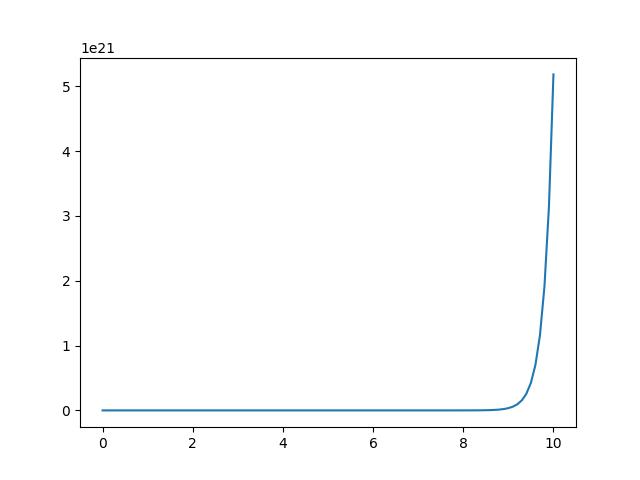
\includegraphics[width=0.8\textwidth]{Images/1st_order_ODE.png}
        \caption{x vs. t plot}
    \end{center}
\end{figure}

\newpage

\section{2$^{nd}$ Order ODE (Classical Harmonic Oscillator - Damping)}
\textbf{THEORY:}
We can split a $2^{nd}$ order differential equation into two coupled $1^{st}$ order equations. For each of the first order equations we can use \texttt{odeint()} to solve.\\
To solve, we need two initial values of $\pmb{x}$ and $\pmb{y}$ and the array for the values of independent variable $\pmb{t}$ (The domain over which we find out $x$ and $y$ at all points).\\
\\
As the function \pmb{\texttt{odeint(func, y0, t)}} can take only three default arguments, we pack two functions \pmb{\texttt{dxdt}} and \pmb{\texttt{dydt}} into one to put in place of \texttt{`func'} and pack two initial values for dependent variables \pmb{\texttt{(x,y)}} into one name to put in place of \texttt{y0}.

\definecolor{LightGray}{gray}{0.9}
\begin{minted}
[frame=lines,baselinestretch=1.2, bgcolor=LightGray]
{python}

import numpy as np
from scipy.integrate import odeint
import matplotlib.pyplot as plt

z=float(input('enter value of "z": '))           #damping factor
k=float(input('enter value of "k": '))           #spring factor
def f(u,t):
    x=u[0]
    y=u[1]
    dxdt=y
    dydt=-z*y-k*x
    return np.array([dxdt,dydt])
u0=[0,1]
t=np.linspace(0,500,10001)
s=odeint(f,u0,t)
print(s)

plt.plot(s[:,0],s[:,1])
plt.show()
plt.plot(t,s[:,0])
plt.show()

\end{minted}


\definecolor{LightGray}{gray}{0.9}
\begin{minted}
[frame=lines,baselinestretch=1.2, bgcolor=LightGray]
{python}

OUTPUT
enter value of "z": 0.02
enter value of "k": 0.49
[[ 0.          1.        ]
 [ 0.04996479  0.99838847]
 [ 0.09981849  0.99555626]
 ...
 [-0.00890059 -0.00249621]
 [-0.00901986 -0.00227428]
 [-0.00912797 -0.00204979]]
\end{minted}

\begin{figure}[H]
    \begin{center}
        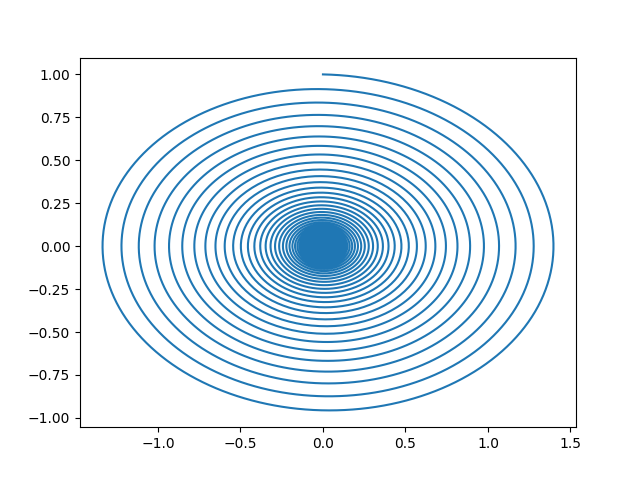
\includegraphics[width=0.8\textwidth]{Images/2nd_order_ODE_2.png}
        \caption{x-y plot}
    \end{center}
\end{figure}
\begin{figure}[H]
    \begin{center}
        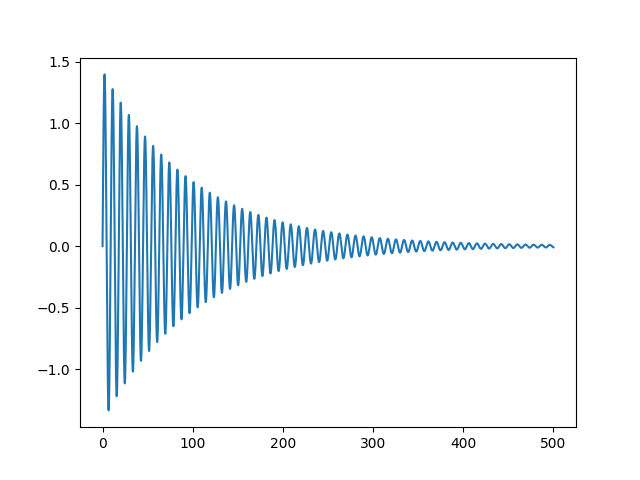
\includegraphics[width=0.8\textwidth]{Images/2nd_order_ODE_3.png}
        \caption{The solution: x vs. t plot}
    \end{center}
\end{figure}

\newpage

\section{Lorentz Attractor Model - Non-Linear Plot}
\textbf{THEORY:}
Consider the following set of three coupled $1^{st}$ order Differential equations:
\begin{gather}
    \frac{dx}{dt}=\sigma(y-x), \\
    \frac{dy}{dt}=x(\rho-z)-y, \\
    \frac{dz}{dt}=xy-\beta z
\end{gather}
Solving these, we arrive at famous Lorentz curves(in the area of Chaos). The values of the parameters that Lorentz used: $\sigma=10, \rho=28, \beta=8/3$

\definecolor{LightGray}{gray}{0.9}
\begin{minted}
[frame=lines,baselinestretch=1.2, bgcolor=LightGray]
{python}

import numpy as np
from scipy.integrate import odeint
import matplotlib.pyplot as plt

def f(u,t):
    x=u[0]
    y=u[1]
    z=u[2]
    dxdt=10*(y-x)
    dydt=x*(28-z)-y
    dzdt=x*y-(8/3)*z
    return np.array([dxdt,dydt,dzdt])
uo=[1,0,0]

t=np.linspace(0,101,100001)
s=odeint(f,uo,t)
print(s)

#plt.plot(t,s[:,0],t,s[:,1],t,s[:,2])  #PLOT OF X(t),Y(t),Z(t)IN SAME GRAPH

plt.plot(s[:,0],s[:,2])                #PLOT OF X(t)vs Z(t)
plt.xlabel("Value of X(t)")
plt.ylabel("Value of Z(t)")
plt.show()

\end{minted}

\definecolor{LightGray}{gray}{0.9}
\begin{minted}
[frame=lines,baselinestretch=1.2, bgcolor=LightGray]
{python}

OUTPUT
[[ 1.00000000e+00  0.00000000e+00  0.00000000e+00]
 [ 9.90092652e-01  2.81247606e-02  1.41229057e-05]
 [ 9.80565956e-01  5.59464679e-02  5.58693144e-05]
 ...
 [-1.03134805e+01 -1.62501880e+01  2.01840013e+01]
 [-1.03734653e+01 -1.63147924e+01  2.02995863e+01]
 [-1.04334924e+01 -1.63785807e+01  2.04165197e+01]]

\end{minted}

\begin{figure}[H]
    \begin{center}
        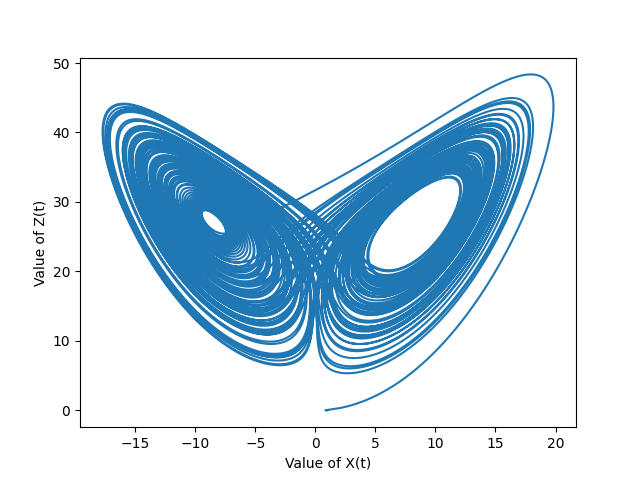
\includegraphics[width=0.8\textwidth]{Images/Non-linear_ODE.png}
        \caption{Lorentz Attractor}
    \end{center}
\end{figure}


\newpage

\section{Gaussian Function}
\textbf{THEORY:}
Consider the Gaussian Integral,
\begin{align}
    \frac{N}{\sigma\sqrt{2\pi}}\int_{-\infty}^{+\infty}e^{-(x-\mu)^2/2\sigma^2}dx = 1
\end{align}
If we want to check this integral, we may choose the integration limits to be as large as possible, which we may essentially call `infinity'.

\definecolor{LightGray}{gray}{0.9}
\begin{minted}
[frame=lines,baselinestretch=1.2, bgcolor=LightGray]
{python}

import numpy as np
from scipy.integrate import odeint
import matplotlib.pyplot as plt

x=np.linspace(-10,10,100)

N=float(input("Enter value of N: "))
sig=float(input("Enter value of sigma: "))
mu=float(input("Enter value of mu: "))

f=lambda x:(N/sig*np.sqrt(2*np.pi))*np.exp((-(x-mu)**2)/(2.0*sig**2))

#print(np.array([x,f(x)]))
plt.plot(x,f(x))
plt.show()

\end{minted}

\begin{figure}[H]
    \begin{center}
        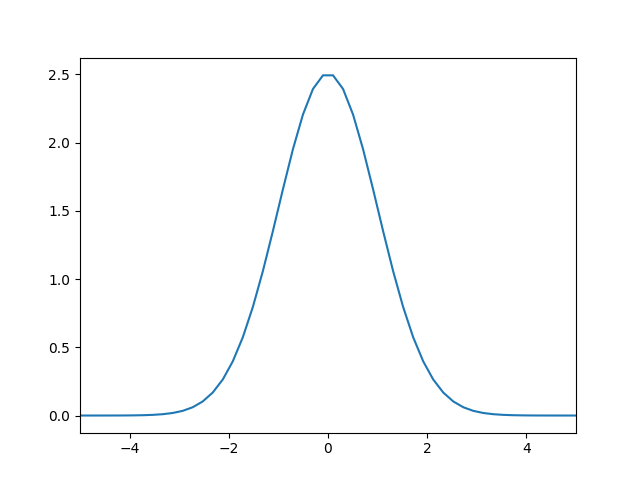
\includegraphics[width=0.8\textwidth]{Images/gaussian_1.png}
        \caption{Gaussian Curve}
    \end{center}
\end{figure}

\newpage

\section{Area Under The Curve Of Gaussian Function}
\textbf{THEORY:}
In \texttt{NumPy}, the constant, \texttt{`inf'} is a floating-point representation of positive infinity. [We can check \texttt{NumPy/SciPy} documentation for all the available constants, \texttt{pi, nan, inf} etc.]. Essentially, positive, or negative \texttt{`infinity'} is the largest or smallest number to represent. Python does it dynamically. We input any number; infinity is larger than that. \\
Here, we use \texttt{quad(), simps(), trapz()} functions to integrate the Gaussian function.
\definecolor{LightGray}{gray}{0.9}
\begin{minted}
[frame=lines,baselinestretch=1.2, bgcolor=LightGray]
{python}

import numpy as np
from scipy.integrate import quad,simps,trapz

import matplotlib.pyplot as plt

x=np.linspace(-2,2,200) 

N=float(input("Enter value of N: ")) #NORMALISATION CONSTANT
sig=float(input("Enter value of sigma: ")) #FWMH WIDTH
mu=float(input("Enter value of mu: "))#POSITION OF PEAK

f=lambda x: (N/sig*np.sqrt(2*np.pi))*np.exp((-(x-mu)**2)/(2.0*sig**2))

s1=quad(f,-np.inf,np.inf)
x1=np.linspace(-1,1,101)
s2=simps(f(x1),x1)
s3=trapz(f(x1),x1)
print('INTEGRATION BY QUAD: ',s1)
print('INTEGRATION BY SIMPSON: ',s2)
print('INTEGRATION BY TRAPZ: ',s3)

#print(np.array([x,f(x)]))

plt.plot(x,f(x))
plt.show()

\end{minted}

\definecolor{LightGray}{gray}{0.9}
\begin{minted}
[frame=lines,baselinestretch=1.2, bgcolor=LightGray]
{python}

OUTPUT
Enter value of N: 1
Enter value of sigma: 0.2
Enter value of mu: 0
INTEGRATION BY QUAD:  (6.283185307179587, 4.639297412243715e-08)
INTEGRATION BY SIMPSON:  6.283181703891748
INTEGRATION BY TRAPZ:  6.2831816274494745

\end{minted}

\begin{figure}[H]
    \begin{center}
        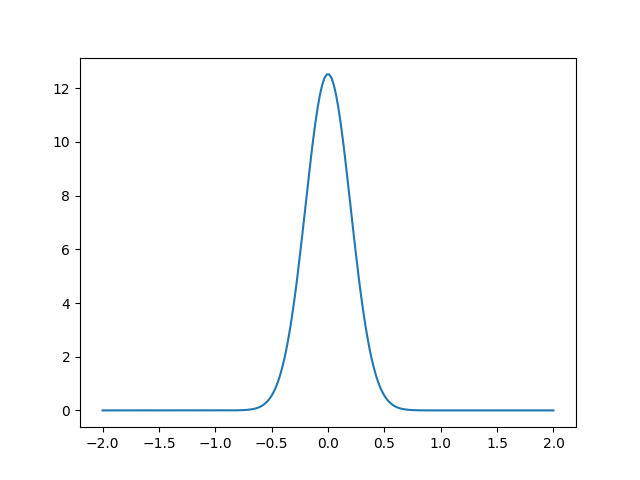
\includegraphics[width=0.8\textwidth]{Images/gaussian_2.png}
        \caption{Another Gaussian Curve}
    \end{center}
\end{figure}

\newpage

\section{Numerically Verifying A Given Gaussian Integral}
\textbf{THEORY:}
To numerically verify the integral,
\begin{align} \label{Gaussian_Integral}
    \int_{-\infty}^{+\infty}e^{(-ax^2+bx+c)}=\sqrt{\frac{\pi}{a}}e^{(\frac{b^2}{4a}+c)}
\end{align}
we make use of \texttt{`inf'} from \texttt{NumPy}, \texttt{quad()} function (alongwith \texttt{simps(), trapz()}) to integrate the LHS of eq.  \ref{Gaussian_Integral} as \texttt{`l(x)'} and see if the result of the integration matches well with the analytical value, i.e, RHS of eq. \ref{Gaussian_Integral} \texttt{`r(x)'}. 
\definecolor{LightGray}{gray}{0.9}
\begin{minted}
[frame=lines,baselinestretch=1.2, bgcolor=LightGray]
{python}

import numpy as np
from scipy.integrate import quad,simps,trapz
import matplotlib.pyplot as plt

a=float(input("Enter value of a: ",)) 
b=float(input("Enter value of b: ",))
c=float(input("Enter value of c: ",))
x=np.linspace(-1,1,101)

l=lambda x: np.exp(-a*x**2+b*x+c)               #LHS of Gaussian Integration
r=lambda x: np.sqrt(np.pi/a)*np.exp((b**2/4*a)+c) #RHS of Gaussian Integration
s1=quad(l,-np.inf,np.inf)
s2=simps(l(x),x)
s3=trapz(l(x),x)

print('VALUE OF LHS INTEGRATION BY QUAD: ',s1)
print('VALUE OF LHS INTEGRATION BY SIMPSON: ',s2)
print('VALUE OF LHS INTEGRATION BY TRAPZ: ',s3)
print('Value of RHS: ', r(x))

\end{minted}

\definecolor{LightGray}{gray}{0.9}
\begin{minted}
[frame=lines,baselinestretch=1.2, bgcolor=LightGray]
{python}

OUTPUT
Enter value of a: 1
Enter value of b: 1
Enter value of c: 1
VALUE OF LHS INTEGRATION BY QUAD:  (6.1864718159341905, 2.0214475437552896e-08)
VALUE OF LHS INTEGRATION BY SIMPSON:  4.598420051234154
VALUE OF LHS INTEGRATION BY TRAPZ:  4.598292642469942
Value of RHS:  6.186471815934188

\end{minted}

\newpage

\section{Dynamical Integration Of Discrete Data}

\definecolor{LightGray}{gray}{0.9}
\begin{minted}
[frame=lines,baselinestretch=1.2, bgcolor=LightGray]
{python}

from scipy.integrate import simps,quad
import numpy as np
import matplotlib.pyplot as plt

x=[0.0,1.0,2.0,3.0,4.0] # x values
y=[0.0,1.0,4.0,9.0,16.0] # corrosponding y values

x1=[]
y1=[]
I=[]

for i in range(len(x)):
    x1.append(x[i])
    y1.append(y[i])
    print (x1,y1)
    I=simps(y1,x1)
    print(I)
plt.plot(x1,y1)  #ploting the Integration values performed manually

#now, original function definition instead of given points
r=np.linspace(0,5) 
plt.plot(r,r**2)

plt.show ()

\end{minted}

\definecolor{LightGray}{gray}{0.9}
\begin{minted}
[frame=lines,baselinestretch=1.2, bgcolor=LightGray]
{python}

OUTPUT
[0.0] [0.0]
0.0
[0.0, 1.0] [0.0, 1.0]
0.5
[0.0, 1.0, 2.0] [0.0, 1.0, 4.0]
2.6666666666666665
[0.0, 1.0, 2.0, 3.0] [0.0, 1.0, 4.0, 9.0]
9.166666666666666
[0.0, 1.0, 2.0, 3.0, 4.0] [0.0, 1.0, 4.0, 9.0, 16.0]
21.333333333333332

\end{minted}

\begin{figure}[H]
    \begin{center}
        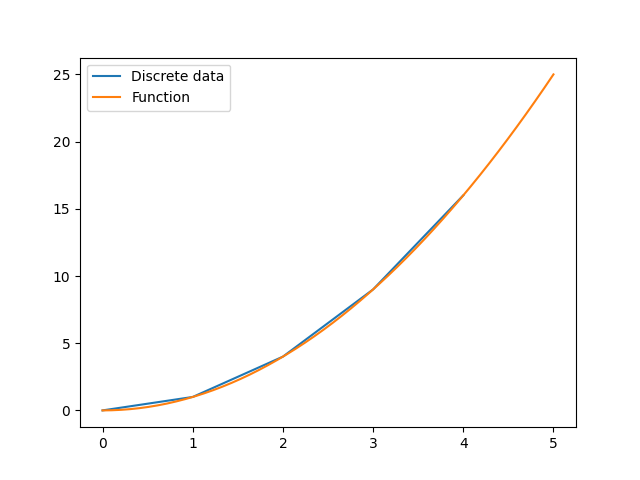
\includegraphics[width=0.8\textwidth]{Images/discrete_integration.png}
        \caption{Plot of Integration of Discrete Data and its Function}
    \end{center}
\end{figure}

\newpage

\section{Gaussian to Delta Function}
\textbf{THEORY:}
\begin{align}
    \int_{-\infty}^{+\infty}g(x)G(x-\mu)dx=g(\mu)
\end{align}
Verifying the above integral by using different limiting representations of $G(x-\mu)$, where $G(x-\mu)$ is a Gaussian function. \\
We use the function:
\begin{align}
    f(x)=(x^2+3x)\frac{N}{\sigma\sqrt{2\pi}}\int_{-\infty}^{+\infty}e^{-(x-\mu)^2/2\sigma^2}dx
\end{align}

\definecolor{LightGray}{gray}{0.9}
\begin{minted}
[frame=lines,baselinestretch=1.2, bgcolor=LightGray]
{python}

import numpy as np
from scipy.integrate import quad,simps,trapz
import matplotlib.pyplot as plt

a=float(input("Give the range of the X axis where the function is to be plotted: "))
x=np.linspace(-a,a,200)
N=float(input("Enter value of N: ")) #NORMALISATION CONSTANT
sig=float(input("Enter value of sigma(sig): ")) #FWHM WIDTH
mu=float(input("Enter value of mu: "))#POSITION OF PEAK

f=lambda x:(x**2+3.0*x)*(N/(sig*np.sqrt(2*np.pi)))*np.exp((-(x-mu)**2)/(2.0*sig**2))
#f=lambda x: (N/(sig*np.sqrt(2*np.pi)))*np.exp((-(x-mu)**2)/(2.0*sig**2))

s1=quad(f,-np.inf,np.inf)
print('INTEGRATION BY QUAD: ',s1)
plt.plot(x,f(x))
plt.show()

\end{minted}

\definecolor{LightGray}{gray}{0.9}
\begin{minted}
[frame=lines,baselinestretch=1.2, bgcolor=LightGray]
{python}

OUTPUT
Give the value of the X axis range where the function is to be plotted: 10
Enter value of N: 1
Enter value of sigma(sig): 0.2
Enter value of mu: 0
INTEGRATION BY QUAD:  (0.04000000000000008, 9.187619849545337e-09)

\end{minted}

\begin{figure}[H]
    \begin{center}
        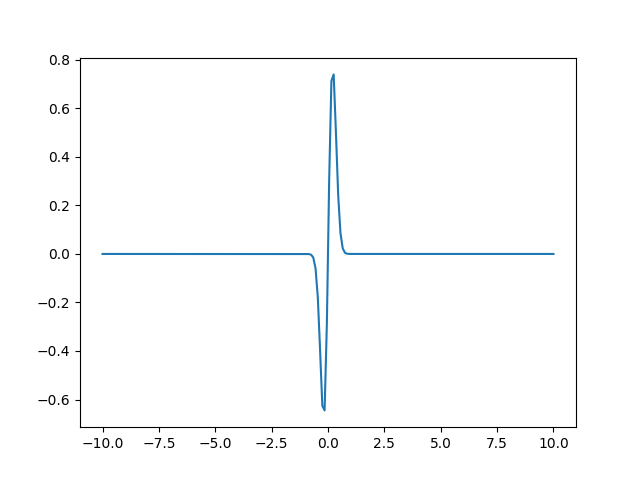
\includegraphics[width=0.8\textwidth]{Images/gaussian_to_delta.png}
        \caption{Plot of the function}
    \end{center}
\end{figure}

\newpage

\section{Plotting of a Delta Function}
\textbf{THEORY:}
Dirac Delta function is type of a peak function which is defined as 
\begin{align}
  \delta(x)=
  \begin{cases}
    +\infty, & x=0, \\
    0, & x\neq 0,
  \end{cases}
\end{align}
Now, to plot the function, we use the same condition as above to define the function. And then \texttt{vectorize()} the function as an array. As we make \texttt{a} sufficiently small, and $\epsilon$ (\texttt{eps}) sufficiently large, the distribution starts to behave like dirac delta function
\definecolor{LightGray}{gray}{0.9}
\begin{minted}
[frame=lines,baselinestretch=1.2, bgcolor=LightGray]
{python}

import numpy as np
from scipy.integrate import quad,simps,trapz
import matplotlib.pyplot as plt

eps=20     #epsilon
a=0.01
delta=lambda x : eps if abs(x)<(a/2) else 0
delta=np.vectorize(delta) #it is used when we plot a piecewise function
x=np.linspace(-2,+2,1000)

plt.plot(x,delta(x))
plt.show()

\end{minted}

\begin{figure}[H]
    \begin{center}
        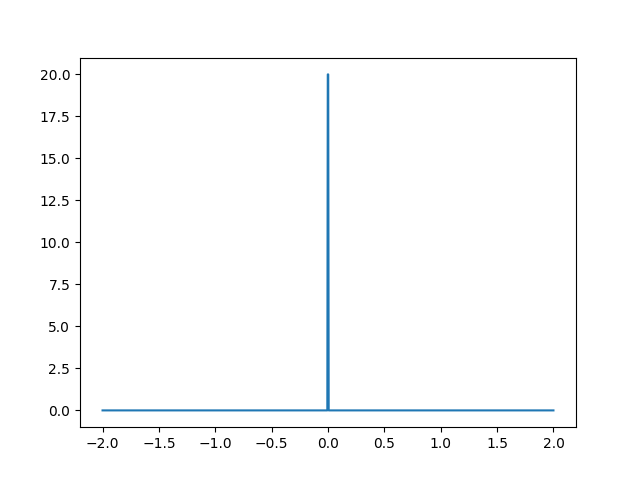
\includegraphics[width=0.8\textwidth]{Images/delta_function.png}
        \caption{Plot of Delta function}
    \end{center}
\end{figure}

\newpage

\section{Legendre Polynomial}
\textbf{THEORY:}
Legendre polynomials are a type of orthogonal polynomials. There are different ways to evaluate a Legendre polynomial, using generating functions, Rodrigues' formula, recurrence relation, Gram-Schmidt orthogonalization etc.\\
Legendre Polynomials (of different orders) satisfy the following differential equation:
\begin{align}
    \frac{d}{dx}[(1-x^2)\frac{d}{dx}P_n(x)]+n(n+1)P_n(x)=0
\end{align}

Rodrigues' formula:
\begin{align}
    P_n(x)=\frac{1}{2^nn!}\frac{d^n}{dx^n}[(x^2-1)^n]
\end{align}

To plot the legendre polynomials, we use the module \texttt{legendre} from \texttt{scipy.special}.

\definecolor{LightGray}{gray}{0.9}
\begin{minted}
[frame=lines,baselinestretch=1.2, bgcolor=LightGray]
{python}

from scipy.special import legendre as l
import numpy as np
import matplotlib.pyplot as plt

x=np.linspace(-1,1,1000)
for i in range(10):
    plt.plot(x,l(i)(x),label="$P_{}(x)$".format({i}))
plt.legend()
plt.show()

\end{minted}

\begin{figure}[H]
    \begin{center}
        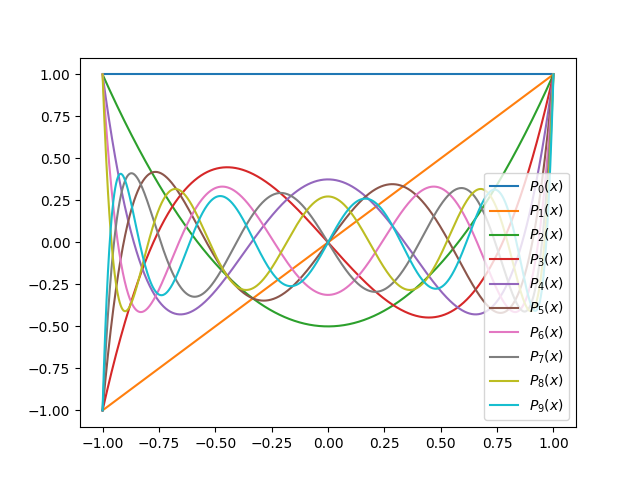
\includegraphics[width=0.8\textwidth]{Images/Legendre_1.png}
        \caption{Legendre Polynomials}
    \end{center}
\end{figure}

\newpage

\section{Legendre Recursion Formula-1}
\textbf{THEORY:}
To plot the given legendre recursion relation, we use the module \texttt{legendre} from \texttt{scipy.special}.
\begin{align}
    (n+1)P_{n+1}(x)=(2n+1)xP_n(x)-n+P_{n-1}(x)
\end{align}

\definecolor{LightGray}{gray}{0.9}
\begin{minted}
[frame=lines,baselinestretch=1.2, bgcolor=LightGray]
{python}
from scipy.special import legendre as l
import numpy as np
import matplotlib.pyplot as plt

x=np.linspace(-1,1,1000)
n=int(input("Enter value of 'n': "))
LHS = (n+1)*l(n+1)(x)
RHS = (2*n+1)*x*l(n)(x)-n*l(n-1)(x)

plt.plot(x,LHS,'*',color="red",label="LHS")
plt.plot(x,RHS,'+',color="cyan",label="RHS")
plt.legend()
plt.show()
\end{minted}

\definecolor{LightGray}{gray}{0.9}
\begin{minted}
[frame=lines,baselinestretch=1.2, bgcolor=LightGray]
{python}
OUTPUT
Enter value of 'n': 4
\end{minted}

\begin{figure}[H]
    \begin{center}
        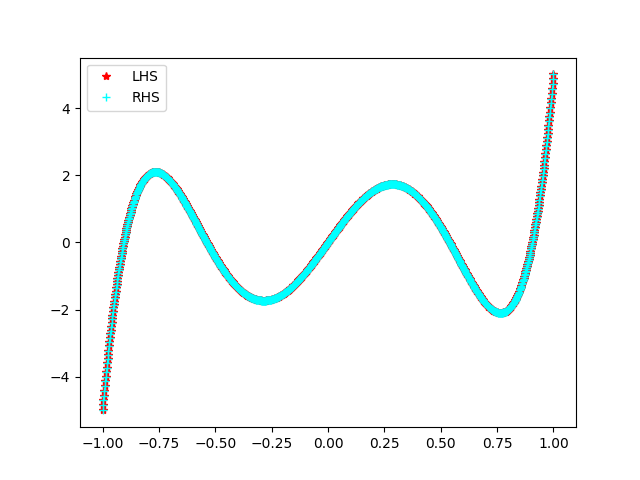
\includegraphics[width=0.8\textwidth]{Images/legendre_recursion_1.png}
        \caption{Plot of the relation}
    \end{center}
\end{figure}

\newpage

\section{Legendre Recursion Formula-2}
\textbf{THEORY:}
To plot the given legendre recursion relation, we use the module \texttt{legendre} from \texttt{scipy.special}.
\begin{align}
    (1-x)^2P\;'_n(x)=(n+1)xP_n(x)-(n+1)P_{n+1}(x)
\end{align}

\definecolor{LightGray}{gray}{0.9}
\begin{minted}
[frame=lines,baselinestretch=1.2, bgcolor=LightGray]
{python}
from scipy.special import legendre as p
import numpy as np
import matplotlib.pyplot as plt

x=np.linspace(-1,1,100)
n=5
LHS = lambda x : (1-x**2)*np.polyder(p(n))(x)
RHS = lambda x : (n+1)*x*p(n)(x)-(n+1)*p(n+1)(x)

plt.plot(x,LHS(x),'*',color="red",label="LHS")
plt.plot(x,RHS(x),'+',color="yellow",label="RHS")
plt.legend()
plt.show()
\end{minted}

\begin{figure}[H]
    \begin{center}
        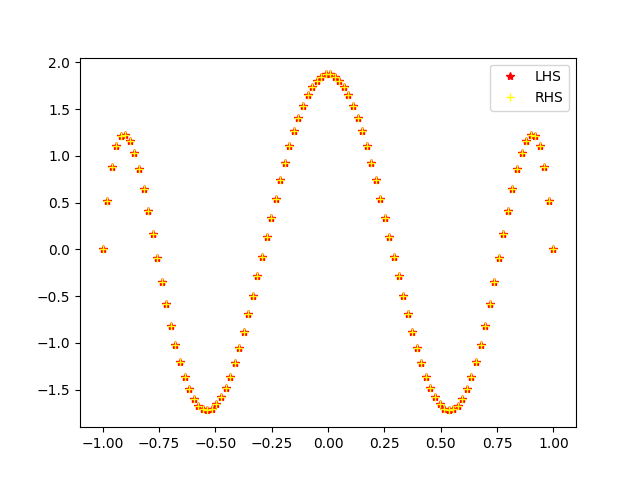
\includegraphics[width=0.8\textwidth]{Images/legendre_recursion_2.png}
        \caption{Plot of the relation}
    \end{center}
\end{figure}

\newpage

\section{Orthogonality of Legendre Polynomial}
\textbf{THEORY:}
To check the Orthogonality relations of Legendre Polynomials, we use the module \texttt{legendre} from \texttt{scipy.special} and \texttt{simps()} from \texttt{scipy.integrate}.
\begin{align}
  \int_{-1}^{1}P_n(x)P_m(x)dx=
  \begin{cases}
    0, & m \neq n, \\
    \frac{2}{2n+1}, & m=n,
  \end{cases}
\end{align}

\definecolor{LightGray}{gray}{0.9}
\begin{minted}
[frame=lines,baselinestretch=1.2, bgcolor=LightGray]
{python}
from scipy.special import legendre as P
import numpy as np
from scipy.integrate import simps as S

n=int(input("Give the value of n: "))
m=int(input("Give the value of m: "))
x=np.linspace(-1.0,1.0,1001)
y=(P(n)(x))*(P(m)(x))
I=S(y,x)
print(I)
\end{minted}

\definecolor{LightGray}{gray}{0.9}
\begin{minted}
[frame=lines,baselinestretch=1.2, bgcolor=LightGray]
{python}
OUTPUT-1
Give the value of n: 5
Give the value of m: 5
0.18181818364742836
\end{minted}

\definecolor{LightGray}{gray}{0.9}
\begin{minted}
[frame=lines,baselinestretch=1.2, bgcolor=LightGray]
{python}
OUTPUT-2
Give the value of n: 5
Give the value of m: 6
0.0
\end{minted}

\newpage

\section{Convolution 1}
\textbf{THEORY:}
Verifying that the convolution of two Gaussian functions is also Gaussian.
\begin{gather}
    f(x)=e^{-(x-2)^2/2} \\
    g(x)=e^{-(x-1)^2/2}
\end{gather}
Convolution Formula:
\begin{align}
    S=\int_{-x}^{+x}f(x-\tau)g(x)d\tau
\end{align}

\definecolor{LightGray}{gray}{0.9}
\begin{minted}
[frame=lines,baselinestretch=1.2, bgcolor=LightGray]
{python}
from scipy.special import legendre as p
import numpy as np
import matplotlib.pyplot as plt
from scipy.integrate import simps

x=np.linspace(-10,10,1000)

f = lambda x: np.exp((-(x-2)**2)/2)
g = lambda x: np.exp((-(x-1)**2)/2)

S = []
for i in range(len(x)):
    t = np.linspace(-x[i],x[i],1000)
    I= simps(f(x[i]-t)*g(x),t)
    S.append(I)
plt.plot(x,S)
plt.show()
\end{minted}

\begin{figure}[H]
    \begin{center}
        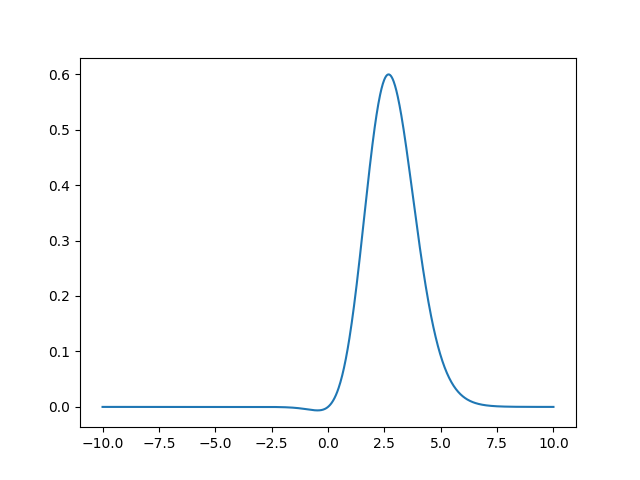
\includegraphics[width=0.7\textwidth]{Images/convolution.png}
        \caption{Plot of convolution of the functions}
    \end{center}
\end{figure}

\newpage

\section{Convolution 2}

\textbf{THEORY:}
Checking the convolution of the two functions:
\begin{gather}
    f(x)=e^{-x} \\
    g(x)=sin(x)
\end{gather}
Convolution Formula:
\begin{align}
    S=\int_{-x}^{+x}f(x-\tau)g(x)d\tau
\end{align}
\vspace{-7mm}
\definecolor{LightGray}{gray}{0.9}
\begin{minted}
[frame=lines,baselinestretch=1.2, bgcolor=LightGray]
{python}
import numpy as np
from scipy.integrate import simps
import matplotlib.pyplot as plt
def f(x): return np.exp(-x)
def g(x): return np.sin(x)
x=np.linspace(0,20,101)
R=[]
for i in range(len(x)):
    t=np.linspace(-x[i],x[i],101)
    S=simps(f(x[i]-t)*g(t),t)
    R.append(S)
actual=(np.exp(-x)+np.sin(x)-np.cos(x))/2
plt.xlabel(r'$x$')
plt.ylabel(r'$R$')
plt.plot(x,R, label="convoluted")
plt.scatter(x,actual, label="actual")
plt.legend()
plt.show()
\end{minted}

\vspace{-7mm}
\begin{figure}[H]
    \begin{center}
        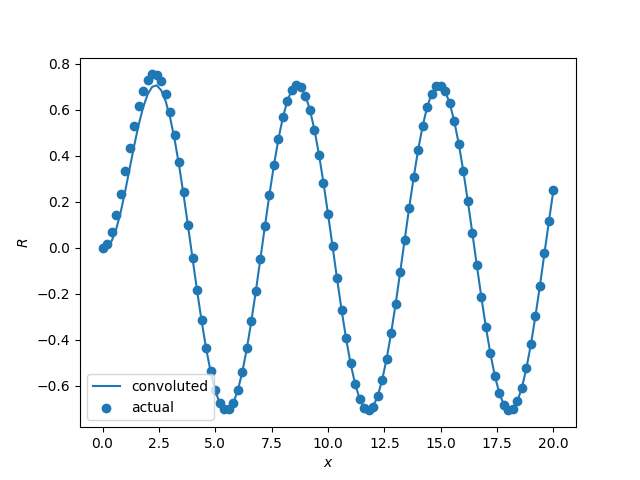
\includegraphics[width=0.7\textwidth]{Images/convolution2.png}
        \caption{Plot of convolution of the functions}
    \end{center}
\end{figure}

\newpage

\section{Bessel Polynomial}

\textbf{THEORY:}
Bessel functions are the solutions of the following second order differential equation,
\begin{align}
    x^2\frac{d^2y}{dx^2}+x\frac{dy}{dx}+(x^2-n^2)y=0
\end{align}
Bessel functions of the first kind,
\begin{align}
    J_n(x)=\sum_{m=0}^{\infty}\frac{(-1)^m}{m! \, \Gamma(m+n+1)}\Big(\frac{x}{2}\Big)^{2m+n}
\end{align}
In the above, $\Gamma(..)$ is a Gamma function. \\
$J_{-n}(x) = (-1)^nJ_n(x)$ \\
Bessel functions of the first kind,
\begin{align}
    Y_n(x)=\frac{J_n(x)cos \, n\pi-J_{-n}(x)}{sin \, n}
\end{align}
To plot the bessel polynomials, we use the module \texttt{jv} from \texttt{scipy.special}.

\definecolor{LightGray}{gray}{0.9}
\begin{minted}
[frame=lines,baselinestretch=1.2, bgcolor=LightGray]
{python}
n=np.arange(0,6,1)
import numpy as np 
from scipy.special import jv
import matplotlib.pyplot as plt 
x=np.linspace(-0,11.0,101)
for i in n:
    plt.plot(x,jv(i,x), label='$J_{}(x)$'.format({i}))
    plt.xlabel('$x$')
    plt.ylabel('$J_n(x)$')
    plt.legend()
plt.show()
\end{minted}
\vspace{-8mm}
\begin{figure}[H]
    \begin{center}
        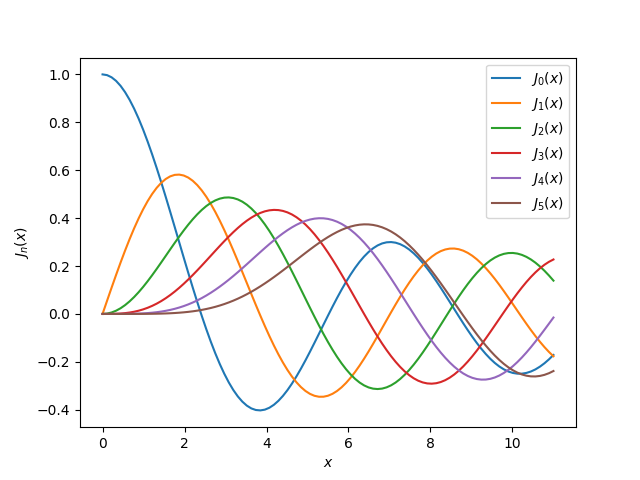
\includegraphics[width=0.8\textwidth]{Images/bessel_1.png}
        \vspace{-5mm}
        \caption{Plot of the Bessel Polynomials}
    \end{center}
\end{figure}

\newpage

\section{Bessel Recursion Relation 1}
\textbf{THEORY:}
To plot the given bessel recursion relation, we use the module \texttt{jv} and \texttt{jvp} from \texttt{scipy.special}:
\begin{align}
    nJ_n(x)+xJ\;'_n(x)=xJ_{n-1}(x)
\end{align}

\definecolor{LightGray}{gray}{0.9}
\begin{minted}
[frame=lines,baselinestretch=1.2, bgcolor=LightGray]
{python}
n=int(input("enter value of n: "))
import numpy as np 
from scipy.special import jv,jvp
import matplotlib.pyplot as plt 
x=np.linspace(-21.0,21.0,101)
L=n*jv(n,x)+x*jvp(n,x)
R=x*jv(n-1,x)
plt.plot(x,L,label="L")
plt.plot(x,R,'*', label="R")
plt.xlabel('$x$')
plt.ylabel('$L & R$')
plt.legend()
plt.show()
\end{minted}

\definecolor{LightGray}{gray}{0.9}
\begin{minted}
[frame=lines,baselinestretch=1.2, bgcolor=LightGray]
{python}
OUTPUT
enter value of n: 5
\end{minted}

\begin{figure}[H]
    \begin{center}
        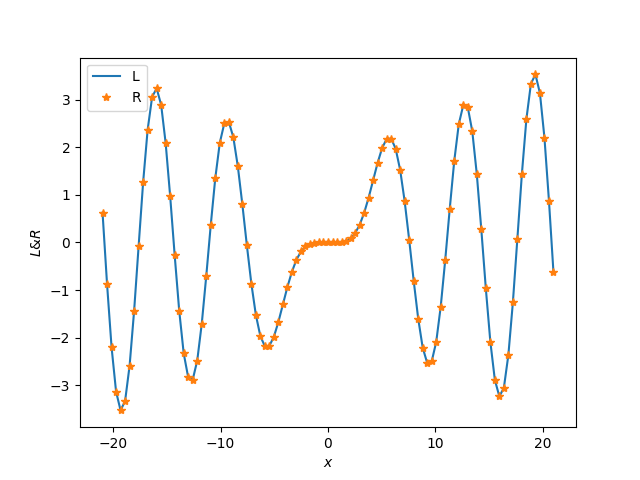
\includegraphics[width=0.8\textwidth]{Images/bessel_recursion_1.png}
        \caption{Plot of the function}
    \end{center}
\end{figure}

\newpage

\section{Bessel Recursion Relation 2}

\textbf{THEORY:}
To plot the given bessel recursion relation, we use the module \texttt{jv} and \texttt{jvp} from \texttt{scipy.special}:
\begin{align}
    x^{-n}J\;'_n(x)-nx^{-n-1}J_n(x)=x^{-n}J_{n+1}(x)
\end{align}

\definecolor{LightGray}{gray}{0.9}
\begin{minted}
[frame=lines,baselinestretch=1.2, bgcolor=LightGray]
{python}
n=int(input("enter value of n: "))
import numpy as np 
from scipy.special import jv,jvp
import matplotlib.pyplot as plt 
x=np.linspace(-21.0,21.0,101)
L=(x**(-n))*jvp(n,x)-n*x**(-n-1)*jv(n,x)
R=-x**(-n)*jv(n+1,x)
plt.plot(x,L,label="L")
plt.plot(x,R,'*', label="R")
plt.xlabel('$x$')
plt.ylabel('$L & R$')
plt.legend()
plt.show()
\end{minted}

\definecolor{LightGray}{gray}{0.9}
\begin{minted}
[frame=lines,baselinestretch=1.2, bgcolor=LightGray]
{python}
OUTPUT
enter value of n: 5
\end{minted}

\begin{figure}[H]
    \begin{center}
        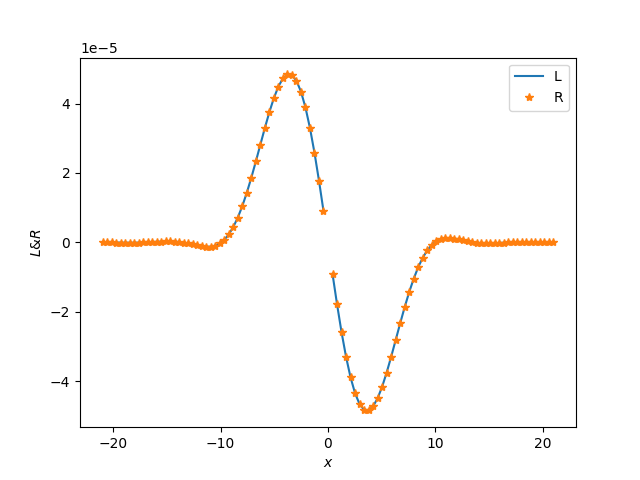
\includegraphics[width=0.8\textwidth]{Images/bessel_recursion_2.png}
        \caption{Plot of the function}
    \end{center}
\end{figure}

\newpage

\section{Orthogonality of Bessel Polynomial}

\textbf{THEORY:}
To check the Orthogonality relations of Bessel Polynomials, we use the module \texttt{jv} from \texttt{scipy.special}, \texttt{root} from \texttt{scipy.optimize} to find the actual roots and \texttt{quad()} from \texttt{scipy.integrate} for integrating the orthogonality relation.
\begin{align}
  \int_{0}^{1}xJ_n(ax)J_n(bx)dx=
  \begin{cases}
    0, & a \neq b, \\
    \frac{(J_{n+1}(a))^2}{2}, & a=b,
  \end{cases}
\end{align}

\definecolor{LightGray}{gray}{0.9}
\begin{minted}
[frame=lines,baselinestretch=1.2, bgcolor=LightGray]
{python}
import numpy as np
from scipy.optimize import root
from scipy.special import jv
import matplotlib.pyplot as plt
from scipy.integrate import quad
x=np.linspace (0,20,1001)
n=int(input('enter the value of n='))
def f(x): return jv(n,x)
plt.hlines(0,0,20)
plt.grid()
plt.plot(x,f(x))
plt.xlabel('$x$')
plt.ylabel('$f(x)$')
plt.show()
a=float(input('enter guessroot1: '))
b=float(input('enter guessroot2: '))
c=float(input('enter guessroot3: '))
S=root(f,np.array([a,b,c])).x
print("actual roots are: ", S)

a=float(input('enter value of a: '))
b=float(input('enter value of b: '))
L= lambda x: x*jv(n,a*x)*jv(n,b*x)
R= (jv(n+1,a)**2)/2
I=quad(L,0,1)[0]
print("LHS: ",I,"RHS: ",R if a==b else 0)
\end{minted}

\definecolor{LightGray}{gray}{0.9}
\begin{minted}
[frame=lines,baselinestretch=1.2, bgcolor=LightGray]
{python}
OUTPUT
enter the value of n=5
\end{minted}

\begin{figure}[H]
    \begin{center}
        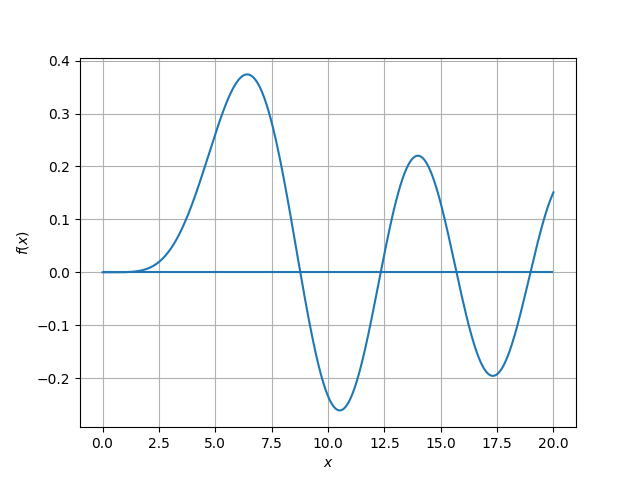
\includegraphics[width=0.8\textwidth]{Images/bessel_orthogonality.png}
        \caption{Plot of the function}
    \end{center}
\end{figure}

\definecolor{LightGray}{gray}{0.9}
\begin{minted}
[frame=lines,baselinestretch=1.2, bgcolor=LightGray]
{python}
enter guessroot1: 8
enter guessroot2: 12
enter guessroot3: 15
actual roots are:  [ 8.77148382 12.3386042  15.70017408]
enter value of a: 8.77
enter value of b: 8.77
LHS:  0.03012916904096064 RHS:  0.03018011768723782
\end{minted}

\newpage

\section{Fourier Series}

\textbf{THEORY:}
Fourier expansion of a function $f(x\;'$ is given by:
\begin{align}
    f(x\;')=\frac{a_0}{2}+\sum_{n=1}^{\infty}a_ncos(nx\;')+\sum_{n=1}^{\infty}b_nsin(nx\;')
\end{align}
The Fourier coefficients are given by the integrals:
\begin{gather}
    a_0=\frac{1}{\pi}\int_{-\pi}^{+\pi}f(x)dx \\
    a_n=\frac{1}{\pi}\int_{-\pi}^{+\pi}f(x)cos(nx)dx \\
    b_n=\frac{1}{\pi}\int_{-\pi}^{+\pi}f(x)sin(nx)dx 
\end{gather}


\definecolor{LightGray}{gray}{0.9}
\begin{minted}
[frame=lines,baselinestretch=1.2, bgcolor=LightGray]
{python}
import numpy as np
from scipy.integrate import simps 
import matplotlib.pyplot as plt 

def f(x): return x**2

n=1
xp=np.linspace(0,20,1001)
x=np.linspace(-np.pi, np.pi, 100)
a0=(1/np.pi)*simps(f(x),x)

def a(n): return (1/np.pi)*simps(f(x)*np.cos(x),x)
def b(n): return (1/np.pi)*simps(f(x)*np.sin(x),x)

s=0.5*a0

R=[]
for i in xp:
    for n in range(1,100):
        s=s+a(n)*np.cos(n*i)+b(n)*np.sin(n*i)
    R.append(s)
plt.plot(xp,R)
plt.xlabel('$x$')
plt.ylabel('$R$')
plt.show()
\end{minted}

\begin{figure}[H]
    \begin{center}
        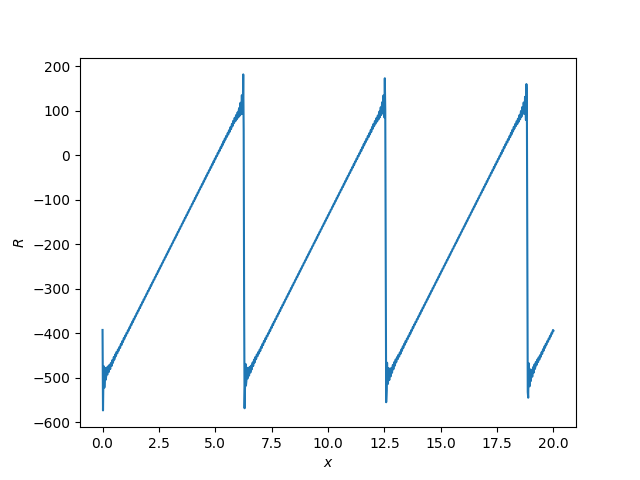
\includegraphics[width=0.8\textwidth]{Images/Fourier.png}
        \caption{Plot of the function}
    \end{center}
\end{figure}

\newpage

\section{Fourier Series of Square, Sawtooth and Triangular Waves}
\textbf{THEORY:} \\
We demonstrate Fourier series over some piecewise continuous functions such as \texttt{square} wave, \texttt{sawtooth} wave and \texttt{triang} wave from the \texttt{scipy.signal} module.

\definecolor{LightGray}{gray}{0.9}
\begin{minted}
[frame=lines,baselinestretch=1.2, bgcolor=LightGray]
{python}
from scipy.signal import square,sawtooth,triang
import matplotlib.pyplot as plt
import numpy as np
from scipy.integrate import simps 

L=100
f=5.0           #f=frequency, n=no. of terms
x=np.linspace(0,L,10000)

yarray=[square(2*np.pi*f*x/L), sawtooth(2*np.pi*f*x/L), triang(10000)]
i=1
labels=["Square", "Sawtooth", "Triangular"]
for y,j in zip(yarray,labels):
    a0=(2/L)*simps(y,x)
    def a(n): return (2/L)*simps(y*np.cos(2*np.pi*n*x/L),x)
    def b(n): return (2/L)*simps(y*np.sin(2*np.pi*n*x/L),x)
    s=0.5*a0
    s=s+sum([a(k)*np.cos(2*np.pi*k*x/L)+b(k)*np.sin(2*np.pi*k*x/L) for k in 
    range(1,101)])
    plt.subplot(2,2,i)
    plt.plot(x,s)
    plt.plot(x,y)
    plt.title(j)
    i=i+1
plt.show()
\end{minted}

\begin{figure}[H]
    \begin{center}
        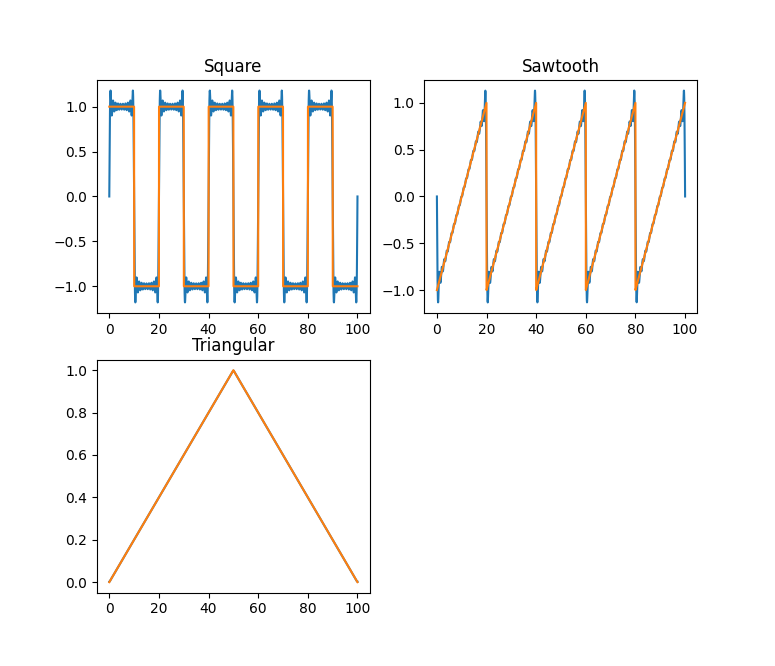
\includegraphics[width=0.8\textwidth]{Images/Fourier_1.png}
        \caption{Plot of the function}
    \end{center}
\end{figure}

\newpage

\section{1D Heat Equation}

\textbf{THEORY:}
1D Diffusion equation or Heat equation is given by:
\begin{align}
    \frac{\partial u}{\partial t}=D^2\frac{\partial^2u}{\partial x^2}
\end{align}
It can reduced to the following form using \textit{Schmidt method} (Eulerian Scheme) for simplifying the numerical calculation:
\begin{align}
    u_j^{i+1}=u_j^i + r(u_{j+1}^i - 2u_j^i +u_{j-1}^i)
\end{align}
where, $0<r<1/2$, for computer analysis, most often, the choice is, $r=1/4$.

\definecolor{LightGray}{gray}{0.9}
\begin{minted}
[frame=lines,baselinestretch=1.2, bgcolor=LightGray]
{python}
import matplotlib.pyplot as plt
import numpy as np
from scipy.integrate import simps 

x=np.linspace(0,1,101)
u=np.zeros(101)
u[50]=1
for i in range(100):        #Time Loop
    for j in range(1,100):
        u[j] += (u[j-1] - 2*u[j] + u[j+1])/4.0
plt.plot(x,u)
plt.xlabel('length ($x$)')
plt.ylabel('amount of heat($u$)')
plt.show()
\end{minted}

\begin{figure}[H]
    \begin{center}
        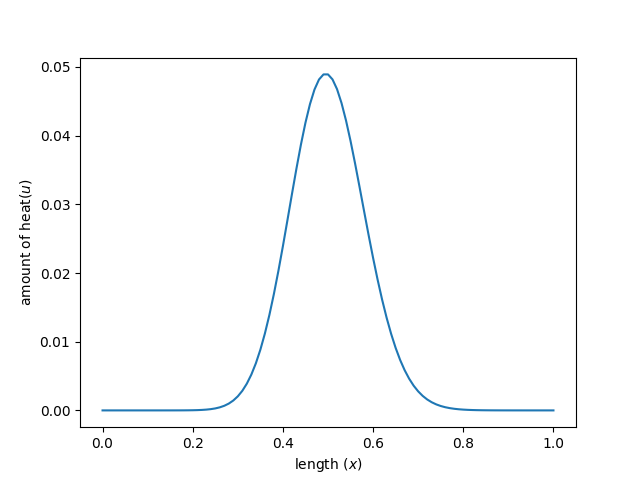
\includegraphics[width=0.8\textwidth]{Images/1d_heat.png}
        \caption{Plot of the function}
    \end{center}
\end{figure}

\newpage

\section{3D Plot of 2D Heat Equation}

\textbf{THEORY:}
2D Diffusion equation or Heat equation is given by:
\begin{align}
    \frac{\partial u}{\partial t}=\frac{\partial^2u}{\partial x^2}+\frac{\partial^2u}{\partial y^2}
\end{align}
It can reduced to the following recursion relation for simplifying the numerical calculation:
\begin{align}
    u_{i,j}^{t+1}=u_{i,j}^t + \frac{(u_{i+1,j}^t + u_{i-1,j}^t + u_{i,j+1}^t + u_{i,j-1}^t - 4u_{i,j}^t)}{4}
\end{align}

\definecolor{LightGray}{gray}{0.9}
\begin{minted}
[frame=lines,baselinestretch=1.2, bgcolor=LightGray]
{python}
import matplotlib.pyplot as plt
import numpy as np
from scipy.integrate import simps 
from matplotlib import cm 

x=np.linspace(0,1,101)
y=np.linspace(0,1,101)
u=np.zeros((101,101))
u[50,50]=1.0     #IC: Heating at middle

for t in range(1000):           #Time Loop
    for i in range(100):        
        for j in range(1,100):
            u[i,j] += (u[i+1,j] + u[i-1,j] + u[i,j+1] + u[i,j-1] - 4*u[i,j])/4.0

X,Y=np.meshgrid(x,y)
plt.axes(projection="3d").plot_surface(X,Y,u, cmap=cm.jet, rstride=1, cstride=1)
plt.show()
\end{minted}

\begin{figure}[H]
    \begin{center}
        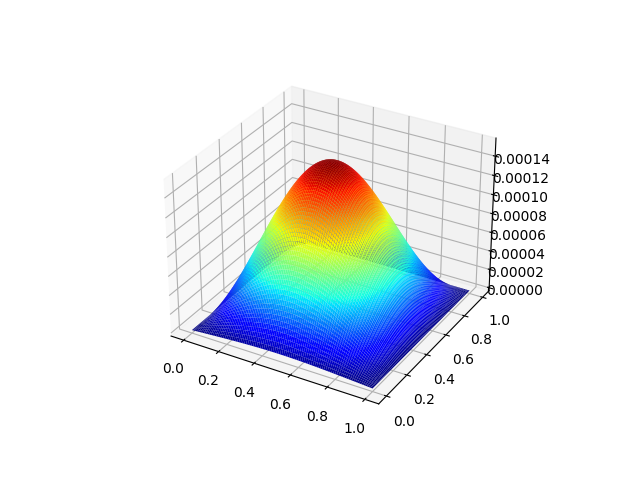
\includegraphics[width=0.8\textwidth]{Images/3d_heat.png}
        \caption{Plot of the function}
    \end{center}
\end{figure}


\end{document}


